 

%%%%%%%%%%%%%%%%%%%%%%%%%%%%%%%%%%
%%% SSI
%%%%%%%%%%%%%%%%%%%%%%%%%%%%%%%%%%

\section{Static Single Information Form (F. Pereira, F. Rastello)}
\begin{frame}
\frametitle{Introduction}
\begin{itemize}
\item \emph{Data-flow analysis}: discover facts (\emph{information}) that are true about a program. Bind to $\textit{Variables} \times \textit{PogramPoints}$.
\item \emph{Static Single Information (SSI) property}: IR such that information of a variable invariant along its whole live-range
\item \emph{$\phi$-functions split live-ranges where reaching definitions collide}: SSA fulfills SSI property for constant analysis. Not for class inference (backward from uses).
\item \emph{Extended SSA}: SSI property for forward analysis flowing from definitions and conditional tests.
\item \emph{SSU}: SSI property for backward analysis flowing from uses
\end{itemize}
\begin{minipage}{0.4\textwidth}
\begin{alertblock}{}
Can we generalize?
\end{alertblock}
\end{minipage}
\end{frame}

\begin{frame}
\frametitle{Sparse Analysis}
\begin{block}{}
  \begin{overprint}
  \onslide<+|handout:+>
    \emph{Non-relational (dense) analysis}: bind information to pairs $\textit{Variables}\times \textit{ProgPoints}$
  \onslide<+|handout:+>
    \emph{Range Analysis}: $[v]^p$ intervals of possible values variable $v$ might assume at program point $p$
  \onslide<+|handout:+>
    \emph{Redundancies}: e.g. $[i]^1 = [i]^2$; because identity transfer function for $[i]$ from $1$ to $2$.  
  \onslide<+|handout:+>
    \emph{Sparse data-flow analysis}: shortcut identity transfer functions by grouping contiguous program points bound to identities into larger regions
  \onslide<+|handout:+>
    \emph{Sparse data-flow analysis}: replace all $[v]^p$ by $[v]$ ($\forall v,\ p\in \textrm{live}(v)$); propagate along def-use chains.
  \end{overprint}
\end{block}%


\vfill
\begin{minipage}[b]{0.2\textwidth}%
\small
\begin{equation*}
\begin{array}[b]{l}
i=0;\\
s=0;\\
\whilett (i<100)\\
\quad i=i+1;\\
\quad s=s+i;\\
\returntt
\end{array}
\end{equation*}
\vspace{1.5cm}
\end{minipage}
\begin{minipage}[b]{0.4\textwidth}%
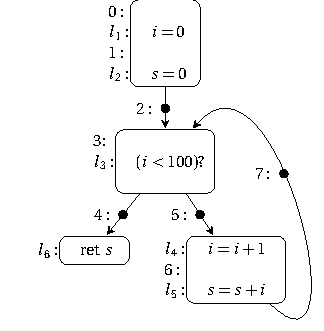
\includegraphics[valign=b,scale=0.85]{range}
\end{minipage}\hfill
\begin{minipage}[b]{0.35\textwidth}
\small
\begin{equation*}
\hspace{-1cm}
\begin{array}[b]{r|l|l}
\textrm{prog. point} & [i] & [s]\\ \hline
0 & \top & \top\\
1 & [0,0] & \top\\
2 & [0,0] & [0,0]\\
3 & [0,100] & [0, +\infty[\\
4 & [100,100] & [0,+\infty[\\
5 & [0,99] & [0,+\infty[\\
6 & [0,100] & [0,+\infty[\\
7 & [0,100] & [0,+\infty[\\
\end{array}
\end{equation*}
\vspace{0.5cm}
\end{minipage}
\end{frame}

\begin{frame}
\frametitle{Partitioned Lattice per Variable Problems}
\begin{exampleblock}{Partitioned Lattice per Variable (PLV) Problem}
\begin{itemize}
\item program variables: $v_i$; program points: $p$; lattice: $\cal L$\\
\item abstract state associated to prog. point $p$: $x^p$\\
\item transfer function associated with $s\in \textit{preds}(p)$: $F^{s,p}$\\
\item constraint system: $x^p = x^p \wedge F^{s,p}(x^s)$ (or eq. $x^p \sqsubseteq  F^{s,p}(x^s)$)\\
\end{itemize}
The corresponding Max. Fixed Point (MFP) problem is a PLV problem iff ${\cal L}={\cal L}_{v_1}\times \dots \times {\cal L}_{v_n}$ where each ${\cal L}_{v_i}$ is the lattice associated with $v_i$ i.e. $x^s=([v_1]^s,\dots,[v_n]^s)$. Thus $F^{s,p}=F^{s,p}_{v_1}\times \dots\times F^{s,p}_{v_n}$ and $[v_i]^p = [v_i]^p \wedge  F^{s,p}_{v_i}([v_1]^s,\dots,[v_n]^s)$.
\end{exampleblock}
\end{frame}

\begin{frame}
\frametitle{Partitioned Lattice per Variable Data-Flow Problem}
\begin{minipage}{0.5\textwidth}
% \vspace{-0.6cm}
{\def\XXX{\vrule height12pt width0pt depth3pt{}}
  \begin{exampleblock}{Range analysis}
\begin{itemize}
\item \XXX $[i]^0 = [i]^0 \only<1|handout:1>{\wedge}\only<2|handout:0>{\cup} \only<1-2|handout:1>{F^{r,0}_i([i]^r, [s]^r)}$
\item \XXX $[i]^1 = [i]^1 \only<1|handout:1>{\wedge}\only<2-|handout:2>{\cup} \only<1-2|handout:1>{F^{l_1}_i([i]^0, [s]^0)}\only<3|handout:2>{[0,0]}$
\item \XXX $[i]^2 = [i]^2 \only<1|handout:1>{\wedge}\only<2-|handout:2>{\cup} \only<1-2|handout:1>{F^{l_2}_i([i]^1, [s]^1)}\only<3|handout:2>{[i]^1}$
\item \XXX $[i]^3 = [i]^3 \only<1|handout:1>{\wedge}\only<2-|handout:2>{\cup} \only<1-2|handout:1>{F^{2,3}_i([i]^2, [s]^2)}\only<3|handout:2>{[i]^2}$
\item \XXX $[i]^3 = [i]^3 \only<1|handout:1>{\wedge}\only<2-|handout:2>{\cup} \only<1-2|handout:1>{F^{7,3}_i([i]^7, [s]^7)}\only<3|handout:2>{[i]^7}$
\item \XXX $[i]^4 = [i]^4 \only<1|handout:1>{\wedge}\only<2-|handout:2>{\cup} \only<1-2|handout:1>{F^{\overline{l_3}}_i([i]^3, [s]^3)}\only<3|handout:2>{\left([i]^3 \only<1|handout:1>{\vee}\only<2-|handout:2>{\cap} [100,+\infty[\right)}$
\item \XXX $[i]^5 = [i]^5 \only<1|handout:1>{\wedge}\only<2-|handout:2>{\cup} \only<1-2|handout:1>{F^{l_3}_i([i]^3, [s]^3)}\only<3|handout:2>{\left([i]^3 \only<1|handout:1>{\vee}\only<2-|handout:2>{\cap} ]-\infty,99[\right)}$
\item \XXX $[i]^6 = [i]^6 \only<1|handout:1>{\wedge}\only<2-|handout:2>{\cup} \only<1-2|handout:1>{F^{l_4}_i([i]^5, [s]^5)}\only<3|handout:2>{\left( [i]^5 + 1\right)}$
\item \XXX $[i]^7 = [i]^7 \only<1|handout:1>{\wedge}\only<2-|handout:2>{\cup} \only<1-2|handout:1>{F^{l_5}_i([i]^6, [s]^6)}\only<3|handout:2>{[i]^6}$
\end{itemize}
\end{exampleblock}}
\end{minipage}%
\hfill
\begin{minipage}{.35\textwidth}
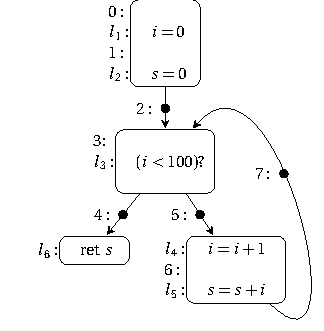
\includegraphics[valign=b,scale=0.85]{range} 
\end{minipage}
\hfill\strut
\end{frame}

\mode<presentation>
\begin{frame}<|handout:0>
\frametitle{The Static Single Information Property}
% SSIfy
\only<1>{\begin{block}{SSIfy (forward)}
Modify the code (split live-ranges) without modifying its semantic s.t. fullfils SSI property
\end{block}}%
% SPLIT
\only<2-3>{\begin{block}{SPLIT}
\only<2>{if $s$ unique pred. of $p\in \textrm{live}(v)$ and such that $F_v^{s,p}\neq \lambda x.\top$ is non-trivial,\\
then $s$ should contain a definition of $v$}%
\only<3>{if $s$ and $t$ two preds of $p$ such that $F_v^{s,p}(Y)\neq F_v^{t,p}(Y)$ ($Y$ a MFP solution),\\
then there must be a \phifun at entry of $p$}
\end{block}}%
% INFO
\only<4>{\begin{block}{INFO}
if $F_v^{s,p} \neq \lambda x.\top$,\\
then $v\in \textrm{live}(p)$
\end{block}}%
% VERSION
\only<5>{\begin{block}{VERSION} 
for each variable $v$, $\textrm{live}(v)$ is a connected component of the CFG.
\end{block}}%
% LINK
\only<6>{\begin{block}{LINK} 
if $F_v^{\textit{inst}}$ depends on some $[u]^s$,\\
then \textit{inst} should contain an use of $u$ live-in at \textit{inst}.
\end{block}}

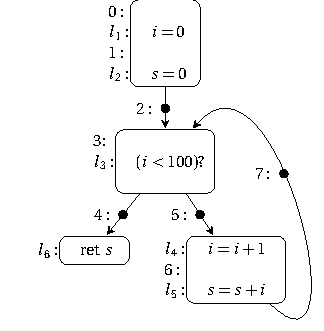
\includegraphics[valign=t,scale=0.85]{range} 
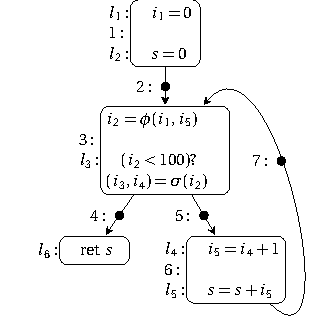
\includegraphics[valign=t,scale=0.85]{range-ssi-onlyi} 
\end{frame}

\mode<handout>
\begin{frame}
\frametitle{The Static Single Information Property}
\begin{block}{SSIfy (forward)}
Modify the code (split live-ranges) without modifying its semantic s.t. fullfils SSI property
\end{block}
% SPLIT
\begin{block}{SPLIT}
  \begin{itemize}
  \item if $s$ unique pred. of $p\in \textrm{live}(v)$ and such that $F_v^{s,p}\neq \lambda x.\top$ is non-trivial,
    then $s$ should contain a definition of $v$
  \item if $s$ and $t$ two preds of $p$ such that $F_v^{s,p}(Y)\neq F_v^{t,p}(Y)$ ($Y$ a MFP solution), then there must be a \phifun at entry of $p$
  \end{itemize}
\end{block}
% INFO
\begin{block}{INFO}
if $F_v^{s,p} \neq \lambda x.\top$,
then $v\in \textrm{live}(p)$
\end{block}
\end{frame}
\begin{frame}
\frametitle{The Static Single Information Property}
\begin{block}{SSIfy (forward)}
Modify the code (split live-ranges) without modifying its semantic s.t. fullfils SSI property
\end{block}
% VERSION
\begin{block}{VERSION} 
for each variable $v$, $\textrm{live}(v)$ is a connected component of the CFG.
\end{block}
% LINK
\begin{block}{LINK} 
if $F_v^{\textit{inst}}$ depends on some $[u]^s$,
then \textit{inst} should contain an use of $u$ live-in at \textit{inst}.
\end{block}
\end{frame}

\mode<all>
\begin{frame}
\frametitle{Special instructions used to split live ranges}
\only<1|handout:1>{\begin{block}{Interior nodes (unique predecessor, unique successor)}
 \[\textit{inst} \ \parallel\  v_1=v'_1 \ \parallel\  \dots \ \parallel\  v_m=v'_m\]
\end{block}}%
\only<2|handout:2>{\begin{block}{joins (multiple predecessors, one successor)}
\centerline{\phifuns}
  \end{block}}%
\only<3|handout:3>{\begin{block}{branch points (one predecessor, mulitple successors)}
\[(l^1:v_1^1, \ldots, l^q:v_1^q) = \sigma(v_1) \ \parallel\  \dots \ \parallel\  (l^1:v_m^1, \ldots, l^q:v_m^q) = \sigma(v_m)\]
\end{block}}%
\vfill
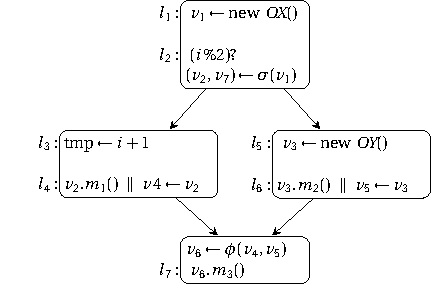
\includegraphics[scale=0.85]{class-inference-ssi}
\end{frame}

\begin{frame}
\frametitle{Propagating Information Forwardly and Backwardly}
\begin{block}{Dense constrained system}
$[v]^p = [v]^p \wedge  F_v^{s,p}([v_1]^s, \dots, [v_n]^s)$
\end{block}
\begin{block}{Sparse SSI constrained system}
$[v] = [v] \wedge  G_v^i([a], \ldots, [z])$ where $a,\dots, z$ are used (resp. defined) at $i$
\end{block}
\begin{minipage}{0.7\textwidth}
\begin{exampleblock}{Proof}
\begin{itemize}
\item coalesce all $[v]^p$ such that $v\in\textrm{live}(p)$ into $[v]$; replace all $[v]^p$ such that $v\not\in\textrm{live}(p)$ by $\top$
\item for each instruction \textit{inst} with uses $a \dots z$, let $G^i_v([a], \dots, [z]) = F^i_v([v_1],\dots, [v_n])$ 
\item remove redundancies 
\end{itemize}
\end{exampleblock}
\end{minipage}
\end{frame}

\begin{frame}
\frametitle{Propagating Information Forwardly and Backwardly}
\begin{minipage}{0.7\textwidth}
\begin{block}{Backward propagation engine under SSI}
{
\def\1{\qquad}
\def\2{\1\1}
\def\3{\2\1}
\def\4{\3\1}
\begin{tabular}{rl}
$_1$ & \textsf{function back\_propagate}(transfer\_functions $\cal G$)\\
$_2$ & \1$\var{worklist} = \emptyset$\\
$_3$ & \1\textsf{foreach } $\var{v} \in \textrm{vars}$: $[v]=\top$\\
$_4$ & \1\textsf{foreach } $\var{i} \in \textrm{insts}$: $\var{worklist}\ +\hspace{-0.3em}= i$\\
$_5$ & \1\textsf{while } $\var{worklist}\neq \emptyset$:\\
$_6$ & \2  \textsf{let } $i \in \var{worklist}$; $\var{worklist}\ -\hspace{-0.3em}= \var{i}$\\
$_7$ & \2 \textsf{foreach } $v \in \var{i.uses}()$:\\
$_8$ & \3    $[v]_{new} = [v] \wedge G_v^i([\var{i.defs}()])$\\
$_9$ & \3    \textsf{if } $[v] \neq [v]_{new}$: \\
$_{10}$& \4      $\var{worklist}\ +\hspace{-0.3em}=\var{v.defs}()$\\
$_{11}$& \4      $[v] = [v]_{new}$\\
\end{tabular}
}
\end{block}
\end{minipage}
\end{frame}

\begin{frame}
\frametitle{Examples of sparse data-flow analyses}
\hspace{-0.5cm}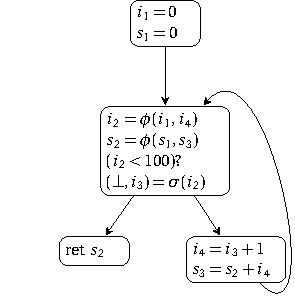
\includegraphics[valign=b,scale=0.95]{range-ssi}\hfill
\begin{minipage}[b]{0.55\textwidth}
\begin{block}{Range analysis (forward from defs \& conds)}
\begin{equation*}
\begin{array}[b]{l|l}
\alert<2|handout:0>{[i_1] \ \cup\hspace{-0.3em}=  [0,0]} & {\only<-2|handout:0>{\alert<1|handout:0>{\emptyset}~~~~~~~~}}\only<3-|handout:1>{\alert<3|handout:0>{[0,0]}}\\

\alert<4|handout:0>{[s_1] \ \cup\hspace{-0.3em}= [0,0]} & {\only<-4|handout:0>{\alert<1|handout:0>{\emptyset}}}\only<5-|handout:1>{\alert<5|handout:0>{[0,0]}}\\

\alert<6|handout:0>{[i_2] \ \cup\hspace{-0.3em}=  [i_1] \cup [i_4]} & {\only<-6|handout:0>{\alert<1|handout:0>{\emptyset}}}\only<7|handout:0>{\alert<7|handout:0>{[0,0]}}\only<8-|handout:1>{[0,100]}\\

[s_2] \ \cup\hspace{-0.3em}= [s_1] \cup [s_3] & {\only<-7|handout:0>{\alert<1|handout:0>{\emptyset}}}\only<8-|handout:1>{[0,+\infty[}\\

[i_3] \ \cup\hspace{-0.3em}= \left([i_2] \cap \left]-\infty,99\right]\right) & {\only<-7|handout:0>{\alert<1|handout:0>{\emptyset}}}\only<8-|handout:1>{[0,99]}\\

[i_4] \ \cup\hspace{-0.3em}= \left([i_3] + 1\right) & {\only<-7|handout:0>{\alert<1|handout:0>{\emptyset}}}\only<8-|handout:1>{[1,100]}\\ 

[s_3] \ \cup\hspace{-0.3em}= \left([s_2] + [i_4]\right) & {\only<-7|handout:0>{\alert<1|handout:0>{\emptyset}}}\only<8|handout:1>{[1,+\infty[}
\end{array}
\end{equation*}
\end{block}
\end{minipage}
\end{frame}

\begin{frame}
\frametitle{Examples of sparse data-flow analyses}
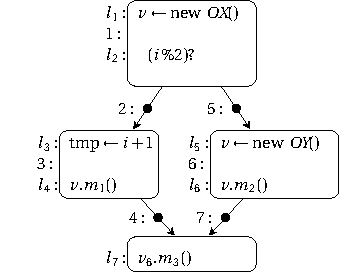
\includegraphics[scale=0.85]{class-inference}
\hfill\begin{minipage}[b]{0.55\textwidth}
\begin{block}{Class inference (backward from uses)}
\begin{equation*}
\begin{array}[b]{c|l}
\textit{prog. point} & [v]\\ \hline
1 & \{m_1, m_3\}\\
2 & \{m_1, m_3\}\\
3 & \{m_1, m_3\}\\
4 & \{m_3\}\\
5 & \top\\
6 & \{m_2, m_3\}\\
7 & \{m_3\}
\end{array}
\end{equation*}
\end{block}
\end{minipage}
\end{frame}

\begin{frame}
\frametitle{Examples of sparse data-flow analyses}
\hspace{-0.8cm}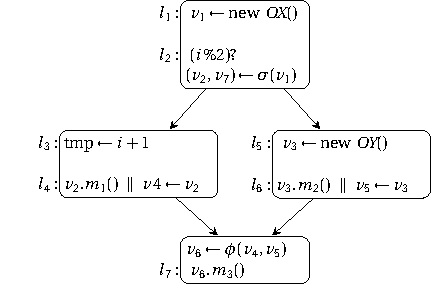
\includegraphics[scale=0.85]{class-inference-ssi}\hfill
\begin{minipage}[b]{0.53\textwidth}
\begin{block}{Class inference (backward from uses)}
\begin{equation*}
\begin{array}[b]{l|l}
[v_7] & \top\\

[v_6] \ \cup\hspace{-0.3em}= \{ m_3 \} & \{ m_3 \}\\

[v_5] \ \cup\hspace{-0.3em}= [v_6] & \{m_3\}\\

[v_4] \ \cup\hspace{-0.3em}= [v_6] & \{m_3\}\\

[v_2] \ \cup\hspace{-0.3em}= \left(\{m_1\} \wedge [v_4]\right) & \{m_1,m_3\}\\

[v_3] \ \cup\hspace{-0.3em}= \left(\{m_2\} \wedge [v_4]\right) & \{m_2,m_3\}\\

[v_1] \ \cup\hspace{-0.3em}= [v_2] & \{m_1,m_3\}\\

[v_1] \ \cup\hspace{-0.3em}= [v_7] & \{m_1,m_3\}
\end{array}
\end{equation*}
\end{block}
\end{minipage}
\end{frame}

\begin{frame}
\frametitle{Examples of sparse data-flow analyses}
\only<1|handout:1>{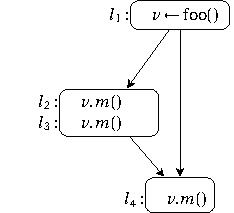
\includegraphics[valign=t,scale=0.85]{null-pointer}}
\only<2|handout:2>{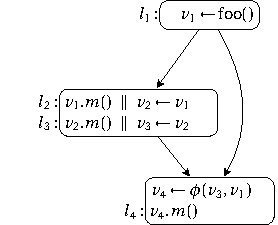
\includegraphics[valign=t,scale=0.85]{null-pointer-ssi}}
\hfill
\begin{minipage}[t]{0.6\textwidth}
\begin{block}{Null pointer (forward from defs \& uses)}
\only<1|handout:1>{~\vspace{2.2cm}}
\only<2|handout:2>{\begin{equation*}
\begin{array}[t]{l|l}
[v_1] \ \wedge\hspace{-0.3em}=  0 & 0\\

[v_2] \ \wedge\hspace{-0.3em}= \nonnull & \nonnull\\

[v_3] \ \wedge\hspace{-0.3em}= \nonnull & \nonnull\\

[v_4] \ \wedge\hspace{-0.3em}= \left([v_3] \wedge [v_1]\right) & 0
\end{array}
\end{equation*}}
\end{block}
\end{minipage}
\end{frame}

\def\SSIfy{\textsf{SSIfy}}
\def\Sdown{\downarrow}
\def\Sup{\uparrow}
\def\SS{{\cal P}}
\def\Out{\textrm{Out}}
\def\In{\textrm{In}}
\def\Defs{\textrm{Defs}}
\def\Def{\textrm{Def}}
\def\Uses{\textrm{Uses}}

\begin{frame}
\frametitle{Splitting strategy}
\begin{block}{Live range splitting strategy $\SS_v = I_\uparrow \cup I_\downarrow$}
$I_\downarrow$: set of points $i$ with forward direction\\
$I_\uparrow$: set of points $i$ with backward direction\\
\end{block}
\vfill
\begin{tabular}{rl}
$_1$& \textsf{function \SSIfy}(var \var{v}, Splitting\_Strategy $\SS_v$)\\
$_2$& \qquad\textsf{split}($v$, $\SS_v$)\\
$_3$& \qquad\textsf{rename}($v$)\\
$_4$& \qquad\textsf{clean}($v$)\\
\end{tabular}
\end{frame}

\begin{frame}
\frametitle{Splitting strategy}
\begin{block}{Range analysis: $\SS_{i} = \{l_1, \Out(l_3), l_4\}_\downarrow$}
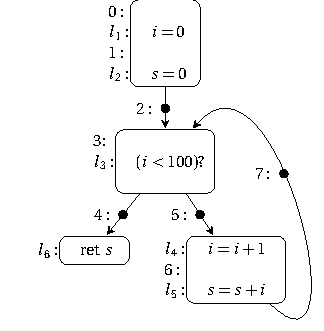
\includegraphics[valign=t,scale=0.85]{range} 
\end{block}
\vfill
\end{frame}

\begin{frame}
\frametitle{Splitting strategy}
\begin{block}{Class inference: $\SS_{v} = \{l_4, l_6,l_7\}_\uparrow$}
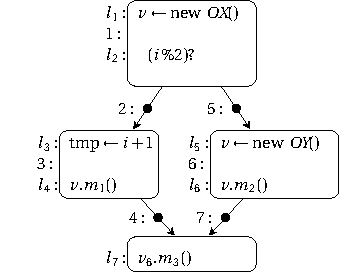
\includegraphics[valign=t,scale=0.85]{class-inference} 
\end{block}
\vfill
\end{frame}

\begin{frame}
\frametitle{Splitting strategy}
\begin{block}{Null pointer: $\SS_{v} = \{l_1, l_2, l_3, l_4\}_\downarrow$}
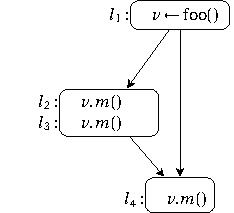
\includegraphics[valign=t,scale=0.85]{null-pointer} 
\end{block}
\vfill
\end{frame}

\begin{frame}
\frametitle{Splitting strategy}
\begin{small}
\renewcommand\arraystretch{1.4}
\begin{tabular}{| c | c |} \hline
{\bf Client} & {\bf Splitting strategy $\SS$} \\ \hline 
Alias analysis, reaching definitions & $\textit{Defs}_\downarrow$ \\ 
cond. constant propagation &  \\ \hline  
Partial Redundancy Elimination & $\textit{Defs}_\downarrow \bigcup \textit{LastUses}_\uparrow$ \\ \hline 
ABCD, taint analysis,  & $\textit{Defs}_\downarrow \bigcup \textit{\Out(Conds)}_\downarrow$ \\ 
range analysis & \\ \hline 
Stephenson's bitwidth analysis & $\textit{Defs}_\downarrow \bigcup \textit{\Out(Conds)}_\downarrow \bigcup \textit{Uses}_\uparrow$  \\ \hline 
Mahlke's bitwidth analysis & $\textit{Defs}_\downarrow \bigcup \textit{Uses}_\uparrow$  \\ \hline 
An's type inference, Class inference & $\textit{Uses}_\uparrow$ \\ \hline 
Hochstadt's type inference & $\textit{Uses}_\uparrow \bigcup \textit{\Out(Conds)}_\uparrow$ \\ \hline 
Null-pointer analysis & $\textit{Defs}_\downarrow \bigcup\textit{Uses}_\downarrow$ \\ \hline
\end{tabular} \end{small}
\end{frame}

\begin{frame}
\frametitle{Splitting live ranges}
\begin{itemize}
\item Split live range of $v$ at each $p\in \SS_v$
\item Split live range where the information collide (join set $\join(I_\downarrow)$ and split set $\Split(I_\uparrow)$)
\item Iterated dominance frontier $\iDF(S)=\join(S\cup \{r\})$ can be computed efficiently (as opposed to $\join(S)$)
\item Iterated post dominance frontier $\ipDF(S)=\join(S\cup \{r\})$ for the reverse CFG
\end{itemize}
\begin{block}{\textsf{function split}(var \var{v}, Splitting\_Strategy
$\SS_v = I_\downarrow \cup I_\uparrow$)}
\only<1-2|handout:0>{\[\left[I_\downarrow\cup \In(\iDF(I_\downarrow))\right]\uncover<2->{\cup\left[I_\uparrow\cup \Out(\ipDF(I_\uparrow))\right]}\]}
\only<3|handout:1>{\[\SS_v\cup \In\left[\iDF(I_\downarrow\cup\left[I_\uparrow\cup \Out(\ipDF(I_\uparrow))\right])\right]\]}
\end{block}
\end{frame}

\begin{frame}
\frametitle{Variable Renaming}
\begin{block}{\sf function rename(var $v$)}
\begin{itemize}
\item traverses the CFG along topological order
\item give a unique version to each definition of $v$
\item stack the versions that dominates the current program point
\item rename each use of $v$ with the version of immediately dominating definition 
\end{itemize}
\end{block}
\end{frame}

\begin{frame}
\frametitle{Dead and Undefined Code Elimination}
\begin{block}{\textsf{clean}(var $v$)}
\begin{itemize}
\item \emph{actual instructions}: instructions originally in the code
\item \emph{SSA graph}: nodes are instructions; edges are def-use chains
\item \emph{active instructions}: instructions connected to an actual instruction
\item simple traversal of the SSA graph from actual instructions that mark active ones
\item remove non-active instructions (inserted phi and sigma functions) 
\end{itemize}
\end{block}
\end{frame}

\begin{frame}
\frametitle{Implementation Details}
\begin{minipage}[t]{0.45\textwidth}
\begin{block}{Implementing $\sigma$-functions}
\hspace{-0.8cm}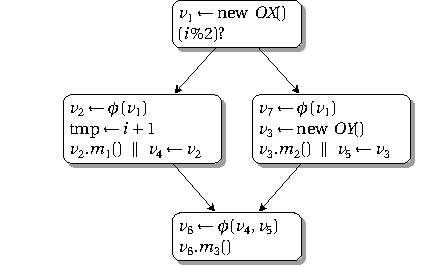
\includegraphics[scale=0.85, valign=t]{class-inference-ssi-out-1}
\end{block}
\end{minipage}\hfill
\begin{minipage}[t]{0.45\textwidth}
\begin{block}{SSI destruction}
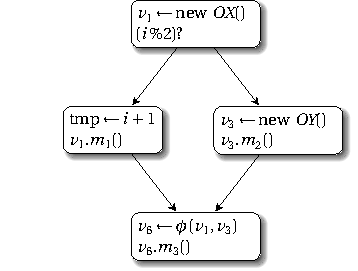
\includegraphics[scale=0.85, valign=t]{class-inference-ssi-out-2}
\end{block}
\end{minipage}
\end{frame}

